% questions.tex —— 2007 年·普通高等学校招生考试·辽宁卷·理科 · 题目内容片段（无答案）
% 由 tools/generate_projects.py 依来源总账自 2007/2007_数学真题_辽宁理_试题.md 生成，勿手改（改源 MD 后重跑）


\gkpart{一、选择题}

\begin{question}
\gkti{1}设集合 $U=\{1,2,3,4,5\}$，$A=\{1,3\}$，$B=\{2,3,4\}$，则 $(\complement_UA)\cap(\complement_UB)=$（　）

（A）$\{1\}$

（B）$\{5\}$

（C）$\{2,4\}$

（D）$\{1,2,4,5\}$

\end{question}
\begin{question}
\gkti{2}若函数 $y=f(x)$ 的反函数图象过点 $(1,5)$，则函数 $y=f(x)$ 的图象必过点（　）

（A）$(1,1)$

（B）$(1,5)$

（C）$(5,1)$

（D）$(5,5)$

\end{question}
\begin{question}
\gkti{3}若向量 $\boldsymbol a$ 与 $\boldsymbol b$ 不共线，$\boldsymbol a\cdot\boldsymbol b\neq0$，且 $\boldsymbol c=\boldsymbol a-\left(\dfrac{\boldsymbol a\cdot\boldsymbol a}{\boldsymbol a\cdot\boldsymbol b}\right)\boldsymbol b$，则向量 $\boldsymbol a$ 与 $\boldsymbol c$ 的夹角为（　）

（A）$0$

（B）$\dfrac{\pi}{6}$

（C）$\dfrac{\pi}{3}$

（D）$\dfrac{\pi}{2}$

\end{question}
\begin{question}
\gkti{4}设等差数列 $\{a_n\}$ 的前 $n$ 项和为 $S_n$，若 $S_3=9$，$S_6=36$，则 $a_7+a_8+a_9=$（　）

（A）$63$

（B）$45$

（C）$36$

（D）$27$

\end{question}
\begin{question}
\gkti{5}若 $\theta\in\left(\dfrac{3\pi}{4},\dfrac{5\pi}{4}\right)$，则复数 $(\cos\theta+\sin\theta)+(\sin\theta-\cos\theta)\mathrm i$ 在复平面内所对应的点在（　）

（A）第一象限

（B）第二象限

（C）第三象限

（D）第四象限

\end{question}
\begin{question}
\gkti{6}若函数 $y=f(x)$ 的图象按向量 $\boldsymbol a$ 平移后，得到函数 $y=f(x+1)-2$ 的图象，则向量 $\boldsymbol a=$（　）

（A）$(-1,-2)$

（B）$(1,-2)$

（C）$(-1,2)$

（D）$(1,2)$

\end{question}
\begin{question}
\gkti{7}若 $m$，$n$ 是两条不同的直线，$\alpha$，$\beta$，$\gamma$ 是三个不同的平面，则下列命题中的真命题是（　）

（A）若 $m\subset\beta$，$\alpha\perp\beta$，则 $m\perp\alpha$

（B）若 $\alpha\cap\gamma=m$，$\beta\cap\gamma=n$，$m\parallel n$，则 $\alpha\parallel\beta$

（C）若 $m\perp\beta$，$m\parallel\alpha$，则 $\alpha\perp\beta$

（D）若 $\alpha\perp\gamma$，$\alpha\perp\beta$，则 $\beta\perp\gamma$

\end{question}
\begin{question}
\gkti{8}已知变量 $x$，$y$ 满足约束条件

\nopagebreak[4]
\[\begin{cases}x-y+2\leqslant0,\\ x\geqslant1,\\ x+y-7\leqslant0,\end{cases}\]

则 $\dfrac yx$ 的取值范围是（　）

（A）$\left[\dfrac95,6\right]$

（B）$\left(-\infty,\dfrac95\right]\cup[6,+\infty)$

（C）$(-\infty,3]\cup[6,+\infty)$

（D）$[3,6]$

\end{question}
\begin{question}
\gkti{9}一个坛子里有编号为 $1$，$2$，$\cdots$，$12$ 的 $12$ 个大小相同的球，其中 $1$ 到 $6$ 号球是红球，其余的是黑球。若从中任取两个球，则取到的都是红球，且至少有 $1$ 个球的号码是偶数的概率为（　）

（A）$\dfrac1{22}$

（B）$\dfrac1{11}$

（C）$\dfrac3{22}$

（D）$\dfrac2{11}$

\end{question}
\begin{question}
\gkti{10}设 $p$，$q$ 是两个命题，$p$：$\log_{\frac12}(|x|-3)>0$，$q$：$x^2-\dfrac56x+\dfrac16>0$，则 $p$ 是 $q$ 的（　）

（A）充分而不必要条件

（B）必要而不充分条件

（C）充分必要条件

（D）既不充分也不必要条件

\end{question}
\begin{question}
\gkti{11}设 $P$ 为双曲线 $x^2-\dfrac{y^2}{12}=1$ 上的一点，$F_1$，$F_2$ 是该双曲线的两个焦点。若 $|PF_1|:|PF_2|=3:2$，则 $\triangle PF_1F_2$ 的面积为（　）

（A）$6\sqrt3$

（B）$12$

（C）$12\sqrt3$

（D）$24$

\end{question}
\begin{question}
\gkti{12}已知 $f(x)$ 与 $g(x)$ 是定义在 $\mathbf R$ 上的连续函数，如果 $f(x)$ 与 $g(x)$ 仅当 $x=0$ 时的函数值为 $0$，且 $f(x)\geqslant g(x)$，那么下列情形不可能出现的是（　）

（A）$0$ 是 $f(x)$ 的极大值，也是 $g(x)$ 的极大值

（B）$0$ 是 $f(x)$ 的极小值，也是 $g(x)$ 的极小值

（C）$0$ 是 $f(x)$ 的极大值，但不是 $g(x)$ 的极值

（D）$0$ 是 $f(x)$ 的极小值，但不是 $g(x)$ 的极值

\end{question}
\gkpart{二、填空题}

\begin{question}
\gkti{13}已知函数 $f(x)=\begin{cases}a\cos x,&x\geqslant0,\\ x^2-1,&x<0,\end{cases}$ 在点 $x=0$ 处连续，则 $a=$\gkblank{}。

\end{question}
\begin{question}
\gkti{14}设椭圆 $\dfrac{x^2}{25}+\dfrac{y^2}{16}=1$ 上一点 $P$ 到左准线的距离为 $10$，$F$ 是该椭圆的左焦点。若点 $M$ 满足 $\overrightarrow{OM}=\dfrac12\left(\overrightarrow{OP}+\overrightarrow{OF}\right)$，则 $|\overrightarrow{OM}|=$\gkblank{}。

\end{question}
\begin{question}
\gkti{15}若一个底面边长为 $\dfrac{\sqrt6}{2}$，侧棱长为 $\sqrt6$ 的正六棱柱的所有顶点都在一个球的面上，则此球的体积为\gkblank{}。

\end{question}
\begin{question}
\gkti{16}将数字 $1$，$2$，$3$，$4$，$5$，$6$ 排成一列，记第 $i$ 个数为 $a_i$（$i=1,2,\cdots,6$）。若 $a_1\neq1$，$a_3\neq3$，$a_5\neq5$，$a_1<a_3<a_5$，则不同的排列方法共有\gkblank{}种。（用数字作答）

\end{question}
\gkpart{三、解答题}

\begin{question}
\gkti{17}已知函数 $f(x)=\sin\left(\omega x+\dfrac{\pi}{6}\right)+\sin\left(\omega x-\dfrac{\pi}{6}\right)-2\cos^2\dfrac{\omega x}{2}$，$x\in\mathbf R$（其中 $\omega>0$）。

（1）求函数 $f(x)$ 的值域；

（2）若对任意的 $a\in\mathbf R$，函数 $y=f(x)$，$x\in(a,a+\pi)$ 的图象与直线 $y=-1$ 有且仅有两个不同的交点，试确定 $\omega$ 的值（不必证明），并求函数 $y=f(x)$，$x\in\mathbf R$ 的单调增区间。

\Needspace{0.4\textheight}
\end{question}
\begin{question}
\gkti{18}如图，在直三棱柱 $ABC-A_1B_1C_1$ 中，$\angle ACB=90^\circ$，$AC=BC=a$，$D$，$E$ 分别为棱 $AB$，$BC$ 的中点，$M$ 为棱 $AA_1$ 上的点，二面角 $M-DE-A$ 为 $30^\circ$。

（1）证明：$A_1B_1\perp C_1D$；

（2）求 $MA$ 的长，并求点 $C$ 到平面 $MDE$ 的距离。
\nopagebreak[4]
\begin{center}% 2007 年辽宁卷理科第 18 题：直三棱柱 ABC-A1B1C1，∠ACB=90°，AC=BC=a；
%   D、E 分别为 AB、BC 中点，M 为 AA1 上一点，二面角 M-DE-A 为 30°。
% 来源 PDF：gaokaomath-src/普通高考/2007/2007辽宁理.pdf
% SHA-256：edddae69cf5dd6502f816cfc494b725ad0cf0cf2e19550bd6b7a3ce31b912bfc
% 原页：2007辽宁理.pdf 第 1 页（A3 三栏）第 3 栏，书页码 389。
% 重绘依据：按原页斜投影与 C1—D、C1—E、M—D、M—E 的虚实线重绘，
%   MA 只画到 AA1 的中部，示意 M 在棱上而非端点。
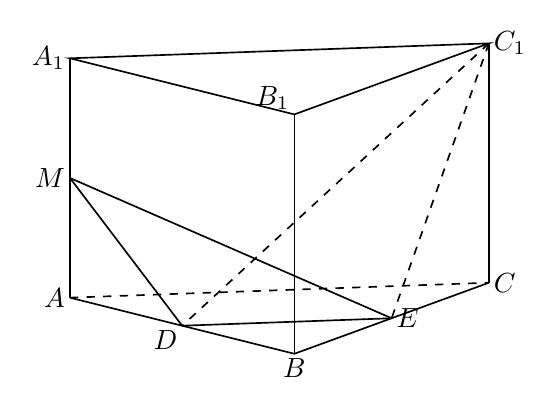
\begin{tikzpicture}[scale=0.95, semithick,
  every node/.style={inner sep=1.5pt}]

  \coordinate (A)  at (0,1.35);
  \coordinate (B)  at (3.0,0.60);
  \coordinate (C)  at (5.6,1.55);
  \coordinate (A1) at (0,4.55);
  \coordinate (B1) at (3.0,3.80);
  \coordinate (C1) at (5.6,4.75);
  \coordinate (D)  at (1.50,0.975);
  \coordinate (E)  at (4.30,1.075);
  \coordinate (M)  at (0,2.95);

  % 被遮挡的底边
  \draw[dashed] (A) -- (C);
  % 可见的底边与侧棱
  \draw (A) -- (B) -- (C);
  \draw (A) -- (A1);
  \draw (B) -- (B1);
  \draw (C) -- (C1);
  % 上底面
  \draw (A1) -- (B1) -- (C1) -- cycle;

  % 题设连线
  \draw[dashed] (C1) -- (D);
  \draw[dashed] (C1) -- (E);
  \draw (M) -- (D);
  \draw (M) -- (E);
  \draw (D) -- (E);

  \node[left] at (A) {$A$};
  \node[below] at (B) {$B$};
  \node[right] at (C) {$C$};
  \node[left] at (A1) {$A_1$};
  \node[above left] at (B1) {$B_1$};
  \node[right] at (C1) {$C_1$};
  \node[left] at (M) {$M$};
  \node[below left] at (D) {$D$};
  \node[right] at (E) {$E$};
\end{tikzpicture}
\end{center}
\nopagebreak[4]
\end{question}
\begingroup
\renewenvironment{question}{\Needspace{0.42\textheight}}{}
\begin{question}
\gkti{19}某企业准备投产一批特殊型号的产品，已知该种产品的成本 $C$ 与产量 $q$ 的函数关系式为 $C=\dfrac{q^3}{3}-3q^2+20q+10$（$q>0$）。该种产品的市场前景无法确定，有三种可能出现的情形，各种情形发生的概率及产品价格 $p$ 与产量 $q$ 的函数关系如下表所示：

\begin{center}
\begin{tabular}{lll}
\toprule
市场情形 & 概率 & 价格 $p$ 与产量 $q$ 的函数关系式 \\
\midrule
好 & $0.4$ & $p=164-3q$ \\
中 & $0.4$ & $p=101-3q$ \\
差 & $0.2$ & $p=70-3q$ \\
\bottomrule
\end{tabular}
\end{center}

设 $L_1$，$L_2$，$L_3$ 分别表示市场情形好、中、差时的利润，随机变量 $\xi_q$ 表示当产量为 $q$ 而市场前景无法确定时的利润。

（1）分别求利润 $L_1$，$L_2$，$L_3$ 与产量 $q$ 的函数关系式；

（2）当产量 $q$ 确定时，求期望 $E\xi_q$；

（3）试问产量 $q$ 取何值时，$E\xi_q$ 取得最大值。

\end{question}
\endgroup
\begin{question}
\gkti{20}已知正三角形 $OAB$ 的三个顶点都在抛物线 $y^2=2x$ 上，其中 $O$ 为坐标原点，设圆 $C$ 是 $\triangle OAB$ 的外接圆（点 $C$ 为圆心）。

（1）求圆 $C$ 的方程；

（2）设圆 $M$ 的方程为 $(x-4-7\cos\theta)^2+(y-7\sin\theta)^2=1$，过圆 $M$ 上任意一点 $P$ 分别作圆 $C$ 的两条切线 $PE$，$PF$，切点为 $E$，$F$，求 $\overrightarrow{CE}\cdot\overrightarrow{CF}$ 的最大值和最小值。

\end{question}
\begin{question}
\gkti{21}已知数列 $\{a_n\}$，$\{b_n\}$ 与函数 $f(x)$，$g(x)$，$x\in\mathbf R$ 满足条件：$b_1=b$，$a_n=f(b_n)=g(b_{n+1})$（$n\in\mathbf N^*$）。

（1）若 $f(x)=tx+1$（$t\neq0$，$t\neq2$），$g(x)=2x$，$f(b)\neq g(b)$，且 $\lim\limits_{n\to\infty}a_n$ 存在，求 $t$ 的取值范围，并求 $\lim\limits_{n\to\infty}a_n$（用 $t$ 表示）；

（2）若函数 $y=f(x)$ 为 $\mathbf R$ 上的增函数，$g(x)=f^{-1}(x)$，$b=1$，$f(1)<1$，证明对任意的 $n\in\mathbf N^*$，$a_{n+1}<a_n$。

\end{question}
\begin{question}
\gkti{22}已知函数 $f(x)=\mathrm e^{2x}-2t(\mathrm e^x+x)+x^2+2t^2+1$，$g(x)=\dfrac12f'(x)$。

（1）证明：当 $t<2\sqrt2$ 时，$g(x)$ 在 $\mathbf R$ 上是增函数；

（2）对于给定的闭区间 $[a,b]$，试说明存在实数 $k$，当 $t>k$ 时，$g(x)$ 在闭区间 $[a,b]$ 上是减函数；

（3）证明：$f(x)\geqslant\dfrac32$。

\end{question}